\section{{\prg Searchspace and Simannfit} - Fitting Experimental Data}\label{simannfit}

In order to fit experimental data a very general concept of fitting program 
has been developed. 
{\prg Perl} has to be installed on the system in order to run
this fitting program.

The program {\prg searchspace\index{searchspace}} is used to cover the parameter space and test
different regions of this space for local minima 
of a specific function {\prg sta(par1, par2 par3 ...)} of
these parameters.. It may be used to 
find good starting values for the program {\prg simannfit\index{simannfit}}.

The program {\prg simannfit\index{simannfit}} uses a simulated annealing algorithm described
in~\cite{kirkpatrick83-671}.
This algorithm does a random walk through the parameter space 
with the aim to fit the parameters to  a minimum of the function {\prg sta}.
  Starting at a set of parameter values (par1, par2, par3) the algorithm
changes these values by a randomly chosen step width (the maximum step width
is specified at the beginning) to (par1', par2', par3').
 The function {\prg sta(par1', par2', par3', ...)} is calculated at
for these new parameter values. The step is accepted if 
$exp([sta(par')-sta(par)]/T)<{\rm a random number out of} [0,1]$.
Otherwise it is rejected. The statistical temperature $T$ involved in this
condition is lowered from step to step as well as the maximum step width allowed.

In the following we describe how to set up the program packages of {\prg McPhase} to
solve a specific fitting problem.
As an example we refer to the fitting of the magnetic 
excitations of CeCu$_2$ in {\prg mcphas/examples/cecu2a/fit}. 

\begin{figure}[hb]\label{safit}
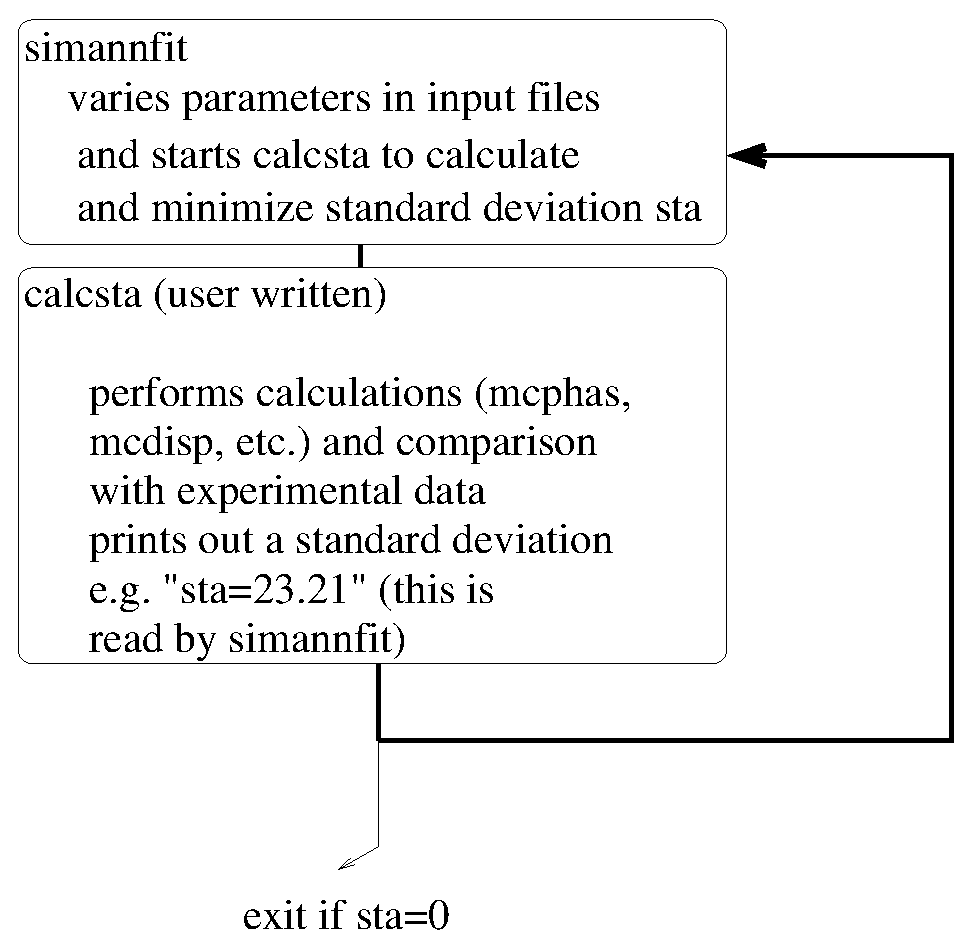
\includegraphics[angle=0,width=0.7\columnwidth]{figsrc/simannfit.eps}
\caption{Layout of the fitting modules.}
\end{figure}


\subsection{Setting up parameter files for fitting}

In order to fit, it is necessary to tell the fitting programs {\prg searchspace\index{searchspace}} and
 {\prg simannfit\index{simannfit}}, which 
parameters in some input files should be varied. Take for instance
the input file {\prg mcphas.jjj}: if you want to vary a parameter, create a file 
{\prg mcphas.jjj.forfit} which is an exact copy of {\prg mcphas.jjj} - in 
this file you substitute the value of the parameter which you want to vary  
 by {\em par}name[value,min,max,xx,stp].
 Here value denotes the starting value, min and max the parameter range, xx an arbitrary
 number (this field will be used by the algorithm to calculate the error of the
 parameter). Stp denotes the maximum step width for this parameter.
Here follows an example:

\begin{enumerate}
\item Original input file {\prg /mcphas/examples/ndba2cu3o7/mcdiff.in}:
{\footnotesize
\begin{verbatim}
...
#
#{atom-file} da[a]  db[b]    dc[c]     dr1[r1]  dr2[r2]  dr3[r3]   <Ma>     <Mb>  <Mc> [mb]
#{corresponding effective fields gjmbHeff [meV]- if passed to mcdiff only these are used 
# for caculation (not the magnetic moments)}
{Nd3p.sipf} 0.50000 0.50000 0.50000 0.50000 0.50000 0.50000 +0.00000 +0.00000 -1.36910  
           corresponding effective fields gjmbHeff [meV]--> +0.00000 +0.00000 -0.07530
{Nd3p.sipf} 0.50000 0.50000 1.50000 0.50000 0.50000 1.50000 +0.00000 +0.00000 +1.36910  
           corresponding effective fields gjmbHeff [meV]--> +0.00000 +0.00000 +0.07530
...
\end{verbatim}
}

	
\item Modified input file{\prg /mcphas/examples/dba2cu3o7/mcdiff.in.forfit}: 
{\footnotesize
\begin{verbatim}
...
#{atom-file} da[a]  db[b]    dc[c]     dr1[r1]  dr2[r2]  dr3[r3]   <Ma>     <Mb>  <Mc> [mb]
#{corresponding effective fields gjmbHeff [meV]- if passed to mcdiff only these are used 
# for caculation (not the magnetic moments)}
{Nd3p.sipf} 0.5000 0.5000 0.5000 0.5000 0.5000 0.5000  0.0000 0.0000 -1.3691  
  corresponding effective fields gjmbHeff [meV]-->     0.0000 parHb %%@
[-2.815596e-003,-2.000000e-002,1.000000e-002,2.762505e-005,4.851325e-003] parHc %%@
[-5.328829e-002,-9.000000e-002,-5.000000e-002,1.614710e-005,4.896285e-003]
{Nd3p.sipf} 0.5000 0.5000 1.5000 0.5000 0.5000 1.5000  0.0000 0.0000 1.3691  
   corresponding effective fields gjmbHeff [meV]-->    0.0000 function[-1*parHb] function[-1*parHc]
...
\end{verbatim}
}

\end{enumerate}

As can be seen constraints on the parameters can be implemented by
substituting the parameter value by {\em function[par}name{\em ]}.
This means for instance, that instead of {\em function[par2a]} the algorithm
uses the parameter {\em par2a} specified at another place of the input file.

\begin{figure}[hb]%h=here, t=top, b=bottom, p=separate figure page
\begin{center}\leavevmode
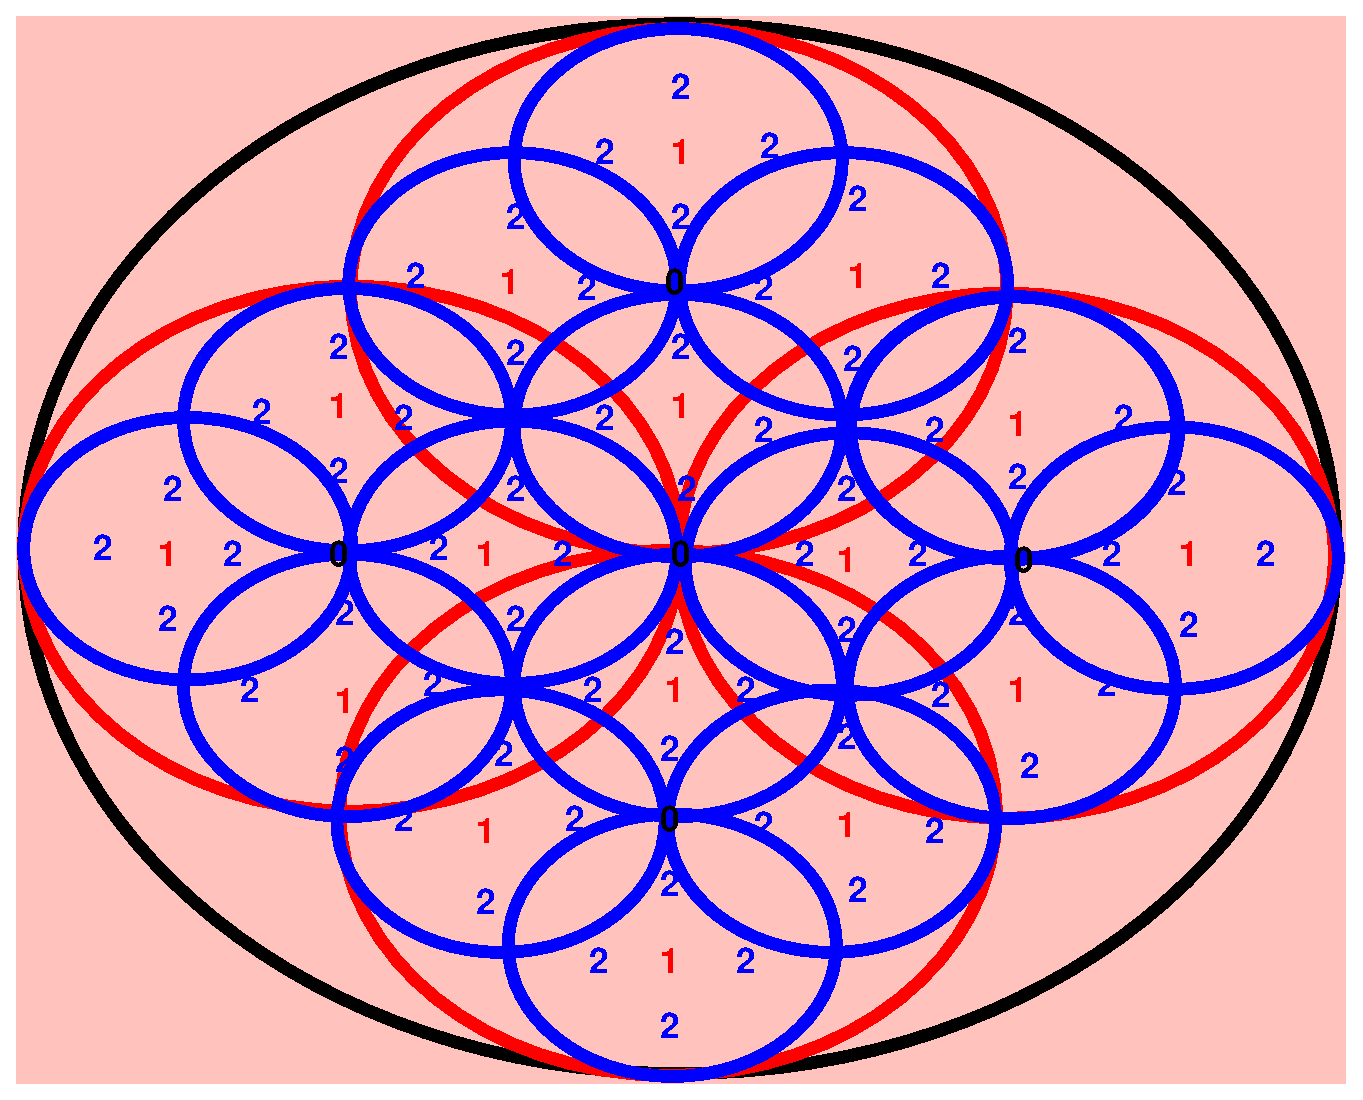
\includegraphics[angle=0, width=0.8\textwidth]{figsrc/searchspace.eps}
\end{center}\label{searchspace}
\caption{Coverage of a two-dimensional parameter space by program {\prg searchspace\index{searchspace}}}
\end{figure}

{\bf What does searchspace/simannfit do with these parameter files ?}

The fitting programs {\prg searchspace\index{searchspace}} and 
{\prg simannfit\index{simannfit}} take the modified file and generate from it an
input file in the original format (using several different
sets of parameters) and call the program
{\prg calcsta} for each parameter set.

\subsection{Telling the fitting program, how to calculate the standard deviation {\prg sta} which should be minimised}


The user must provide a program {\prg calcsta}  (under windows 
it is {\prg calcsta.bat}), which calculates the standard deviation
of some experimental data from model calculated data. This program can
be a bash script such as {\prg /mcphas/examples/cecu2a/fit/calcsta} or just a
very short program such as:


\begin{verbatim}
#!/usr/bin/perl
# do a mcphase simulation. The measured magnetisation data must
# be in directory ./fit/mcphas.fum column 11 12 13.
# the program mcphas\index{mcphas} will compare measured data with calculated
# data and generate an output such as sta=14.3112, which
# contains the standard deviation
system ("mcphas");


\end{verbatim}

... in general the output of this batch (to stdout) must contain a line
such as {\em sta = 4122.32}, which contains the calculated standard
deviation. Note that the programs {\prg McPhas} and {\prg McDisp} always try to
calculate a standard deviation and write such {\em sta = ...} statement
to stdout.
 So it is possible to use these programs. Alternatively (or in addition)
any other program can be called in {\prg calcsta} and calculate the 
standard deviation {\prg sta}.

Before starting a fit it is necessary to test the program {\prg calcsta} by typing
{\prg ./calcsta}. The calculation should run and there must appear an output
the line {\prg sta= ...} on the screen. If this works, a fit may be started.

{\bf Options:} note, that the program {\prg simannfit\index{simannfit}} calls the user written program
{\prg calcsta} with a number as argument, e.g. as {\prg calcsta 21.3}. This number
(i.e. 21.3 in our example) denotes a maximum value of the standard deviation. The
user written program may use this number and stop, when in the summation process
to obtain standard deviation {\prg sta} reaches a value larger than this maximum
number. Using this option is advisable in complex fitting problems in order to
optimise the time of the fitting procedure. Note, that the module {\prg mcphas}
can be used with the option {\prg -stamax 21.3}, which leads to a stop when the value of 
the standard deviation 21.3 is reached. 

\subsection{Starting a parameter space search}

If the program {\prg calcsta} has been set up, the parameter space may be
searched by the program {\prg searchspace\index{searchspace}}. It is started
by the command (in the example you should go to the directory {\prg /mcphas/examples/cecu2a/fit}) 
:

\begin{quote}
 {\prg searchspace 0 mcphas.jjj [and possible other input parameter files]}.
\end{quote}


Note that the user written program {\prg calcsta} has to be in the
directory where {\prg searchspace\index{searchspace}} is started from.
The ''0'' in the command means that the search is started for the first time.
The program generates an output file {\prg searchspace.0} with a list
of parameter sets. This list may be shortened to stop searching 
some regions of the parameter space and subsequently the program may be started
with

\begin{quote}
 {\prg searchspace 1 mcphas.jjj [and possible other input parameter files]}.
\end{quote}


Now the values stored in {\prg searchspace.0} are read and 
the parameter space is searched in more detail and a longer list 
of parameters is stored as {\prg searchspace.1}. This may be again
edited to drop some regions of the parameter space and {\prg searchspace\index{searchspace}}
may be started with {\prg searchspace 2 ...} and so on ....

The program creates new parameter sets from an old set by incrementing/decrementing
each of the parameters subsequently by a small step. In the first level this step
is just equal to a quarter of the parameter range. Going from one level to
 the next this step is halved. Figure ~\ref{searchspace} shows how a two dimensional
 parameter space is covered by this procedure. If all neighbouring points of
 a given point show a larger value of {\prg sta}, then the set is recorded, because it might be
 near a minimum of {\prg sta}. The parameter values are stored in the file
 {\prg results/searchspace.searchspace-level.localminima}.

\subsection{analysing the results of {\prg searchspace}}

The results of a parameter search can be analysed by starting searchspace for example as

\begin{quote}
{\prg searchspace -13 results/searchspace.2.localminima mcphas.jjj [end possible other input files]}.
\end{quote}

In this example the parameter set (line) number 13 is taken from the
 file {\prg results/searchspace.2.localminima}. Obviously this parameter set is the local minimum number 13
from a previous searchspace run with searchspace level 2. Using this input
 searchspace updates {\prg mcphas.jjj} and
other parameter files with this parameter set.
The standard deviation can be recalculated now easily by typing {\prg calcsta}, thereby all
output files are updated and the quality of this parmaeter set can be inspected, e.g. by
making graphs etc.
Note that also the files {\prg *.forfit} are updated with
these parameters (this is useful for a later use with {\prg simannfit}).

\subsection{Starting a fit}

If the program {\prg calcsta} has been set up, the fitting is started
by the command (in the example you should go to the directory {\prg /mcphas/examples/cecu2a/fit}) 
:

\begin{quote}
 {\prg simannfit 10 [-t 1000][-s 100000] mcphas.jjj [and possible other input parameter files]}.
\end{quote}

The ''10'' in the command means that the initial statistical
''temperature'' of the algorithm
is set to 10.  
Option -t sets time limit until program end (in seconds).
Option -s gives maximal number of iteration steps to be done.
Note that the user written program {\prg calcsta} has to be in the
directory where {\prg simannfit\index{simannfit}} is started from.

The program generates for each parameter a histogram file showing the number of occurrences
of a certain parameter value in solutions, where sta decreased.

\subsection{Stopping a fit/parameter space search}

The fitting procedure should be stopped by changing the program {\prg calcsta}, so that it
writes {\prg sta=0} to the standard output (stdout in Linux). Then the fitting
procedure is stopped. The last value of parameters fitted can be found in the
input parameter files.

\subsection{Fitting is an art: some general remarks}

Fitting data is in most cases not a straightforward procedure and requires
a lot of experience and intuition. Even the fitting of a Gaussian to some
experimental data is sometimes difficult and the available algorithms fail,
 if the initial
stepwidths or starting values are not chosen with some care.
This rule holds even more for complex non linear fitting in a large
parameter space. In many cases a simple theoretical model is used
and it is {\bf not} clear at the beginning if this model is able
to describe the data at all. 
So how can reasonable starting parameters be found ? What value
for the statistical temperature has to be chosen ?

One possible way to attack this problem is to monitor the status of a fit
by viewing online its quality when fitting. The value of {\em sta} which is put onto
the screen together with the standard deviation is only a very rudimentary information.
In most cases it is necessary to view the data which is to be fitted graphically and
see how the calculated data matches. It is also advisable to monitor the
standard deviation and how it changes with time. After starting the
fit it should the be possible to judge, if stepwidths should be modified or if
the parameter range was chosen too small or too large etc.

To view online the contents of a file which contains data in column format
the program {\prg display} can be used. To start the display\index{display} of
the file {\em data.dat} with x-axis data in column 1 and y-axis data
in column 2 just type (java has to be installed in order to use this):

display\index{display} 1 2 data.dat

In order to send this data display\index{display} to the background type under Linux:

display\index{display} 1 2 data.dat \&

and under windows:

start display\index{display} 1 2 data.dat


\vspace{1cm}
{\em Exercises:}
\begin{itemize}
\item 
Start the fit example given for the fitting of the magnetic 
excitations of CeCu$_2$ in {\prg mcphas/examples/cecu2a/fit}.
First copy the file {\prg mcphas.jjj.sav} to {\prg mcphas.jjj}
Then start the fit by typing {\prg simannfit 10 mcphas.jjj}.
\item
Stop the fit by editing {\prg calcsta} as described above.
\item 
Copy {\prg mcphas.jjj.fit} to {\prg mcphas.jjj}  and type
{\prg calcsta}. What is the standard-deviation ? 
\item 
In order to fit  crystal field parameters to transition
energies of neutron intensities write a module
{\prg calcsta} for CeCu$_2$ which uses only the program
cfield to calculate the transition matrix elements
and compare them to experimental data.
The section~\ref{addprog} contains some further programs which
might help. 
\end{itemize}
